% Include from a manuscript whose working directory is Overleaf/.
\begin{figure}[tbp]
    \centering
    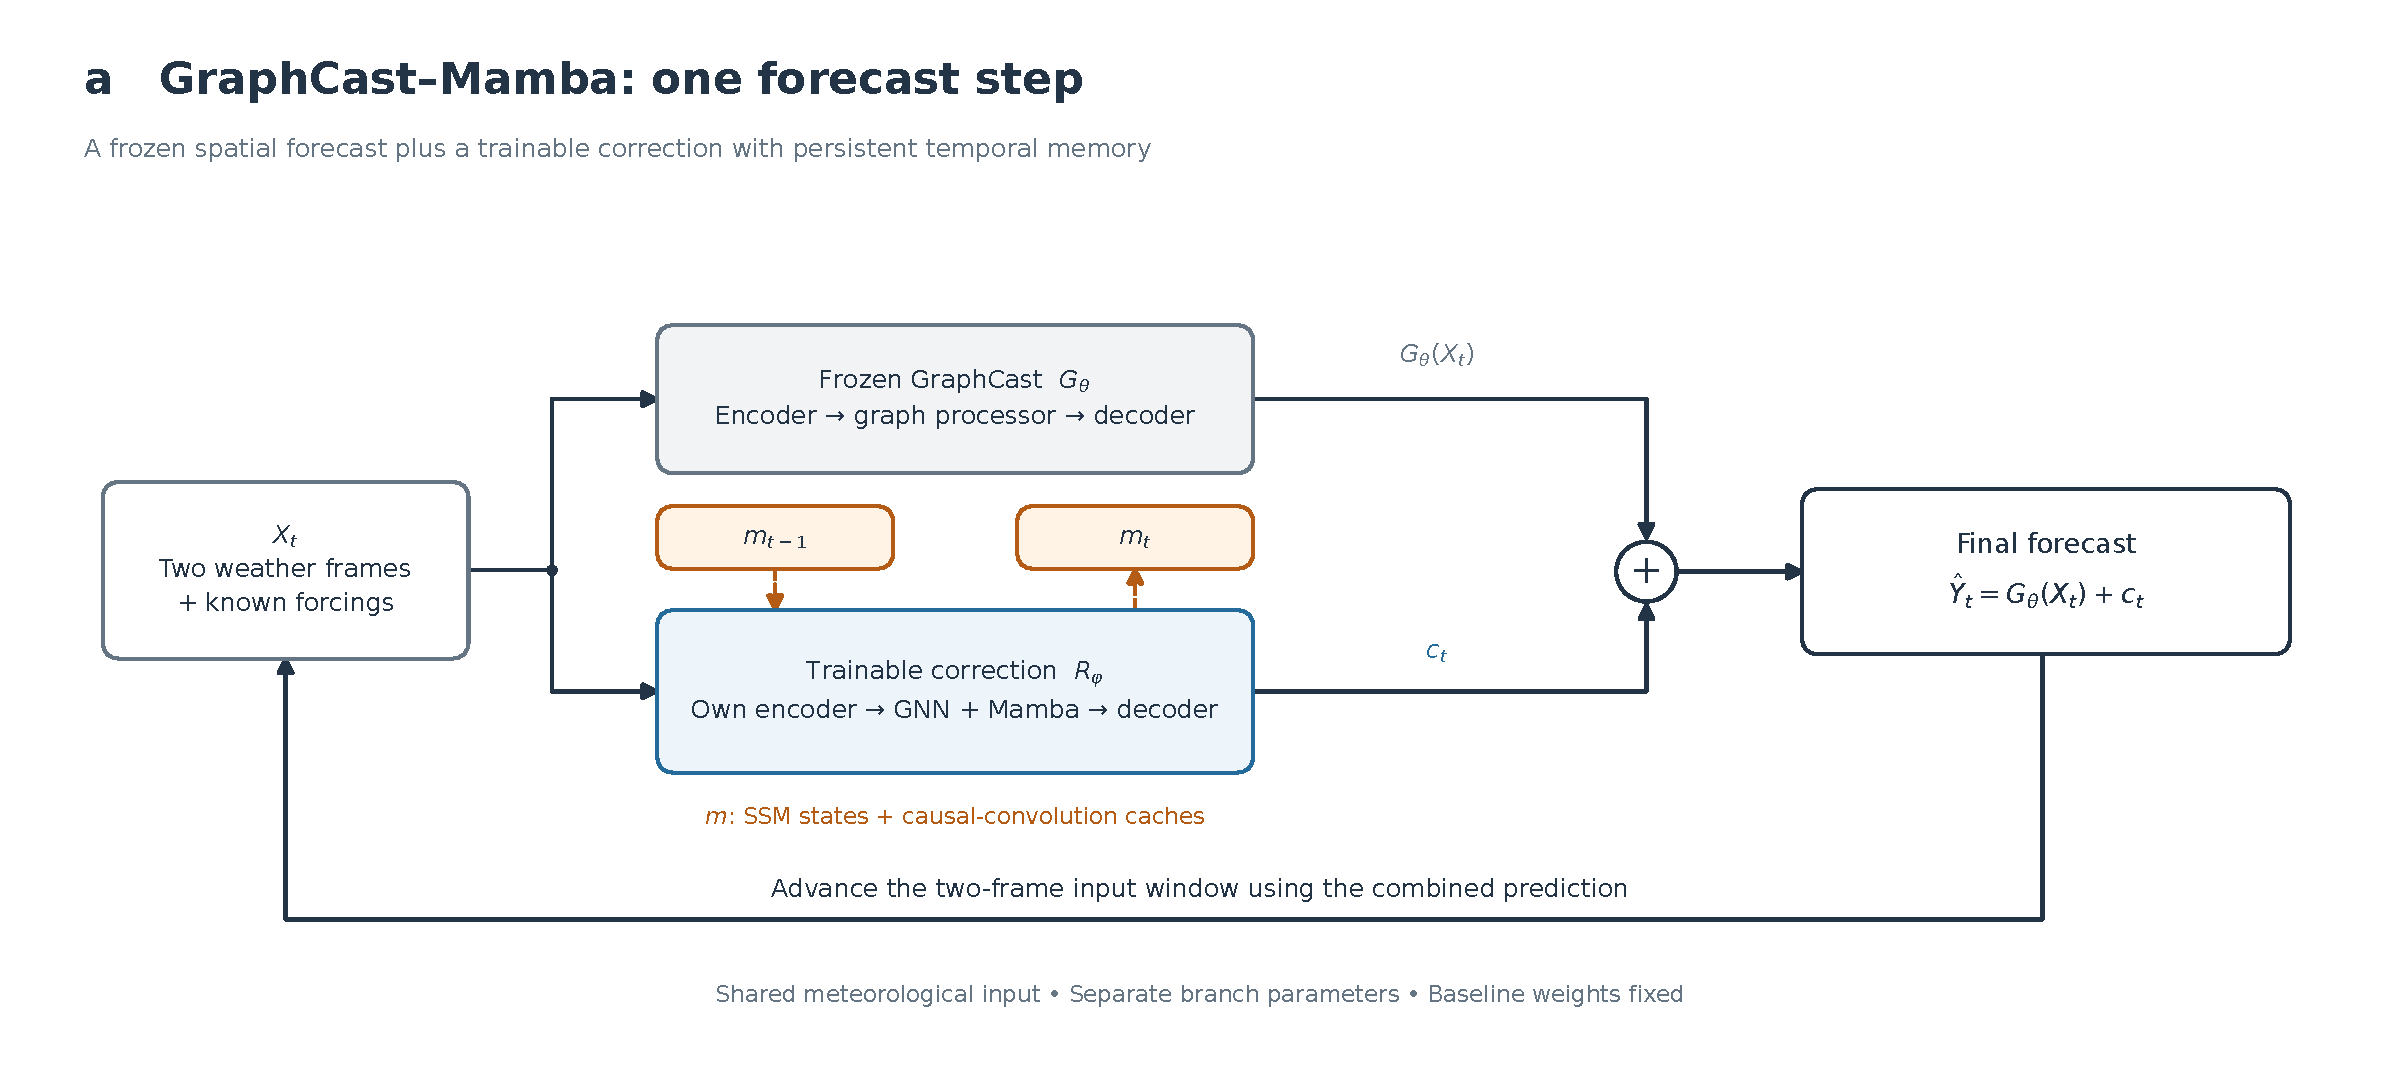
\includegraphics[width=\linewidth]{Pics/gc_mamba_architecture/01_full_model.pdf}
    \caption{GraphCast--Mamba combines a frozen GraphCast forecast with a
    trainable correction. Both branches receive the same meteorological inputs
    and known forcings but have separate parameters. Their outputs are added,
    and the GraphCast--Mamba prediction advances the two-frame weather input window.
    The correction also carries temporal memory $m_t$, comprising Mamba SSM
    states and causal-convolution caches.}
    \label{fig:gc_mamba_full_model}
\end{figure}

\begin{figure}[tbp]
    \centering
    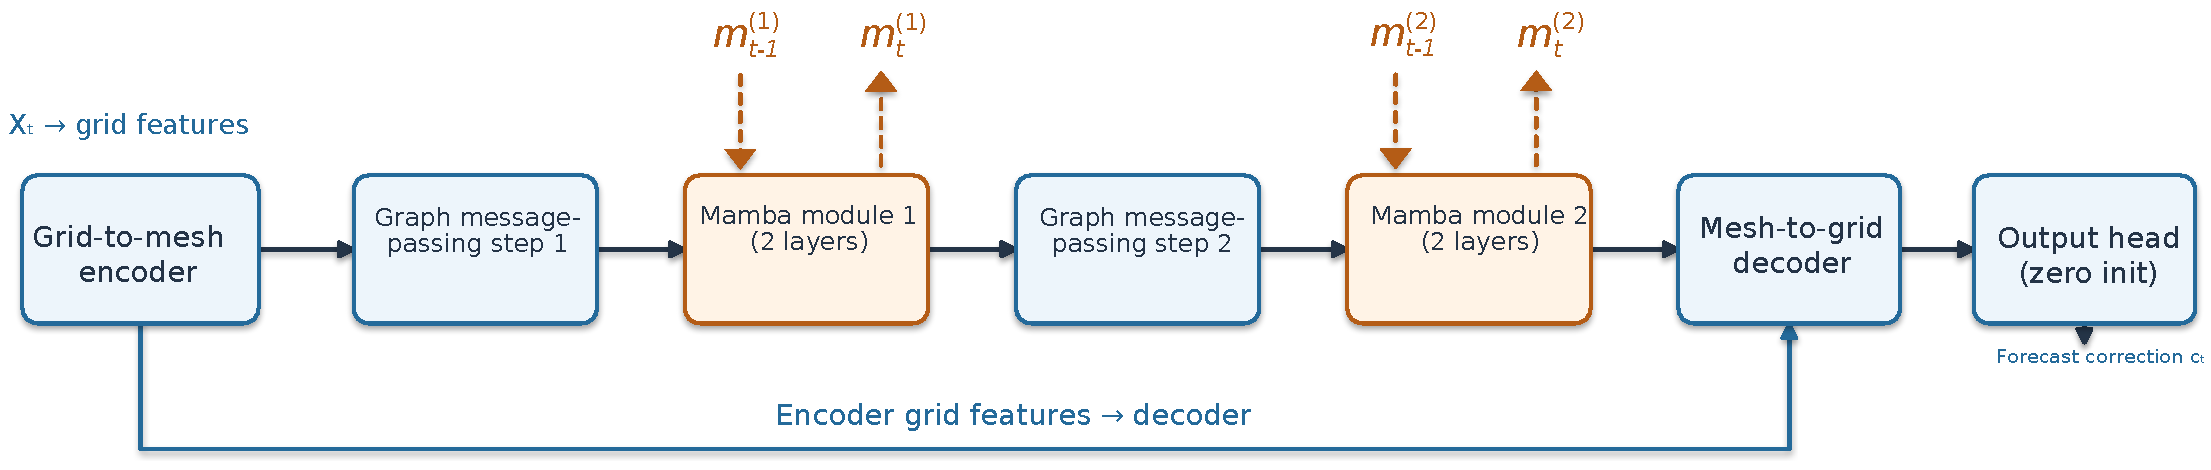
\includegraphics[width=\linewidth]{Pics/gc_mamba_architecture/02_correction_branch.pdf}
    \caption{The trainable Mamba correction branch has its own grid-to-mesh encoder,
    two graph message-passing steps, and a mesh-to-grid decoder followed by a
    zero-initialized output head. Each graph message-passing step is followed by two residual
    Mamba layers, for four recurrent layers in total. Graph processing exchanges
    information between mesh nodes; Mamba processes the temporal sequence at
    each node with shared parameters and separate memory. Each stage's memory
    bundle includes both layers' SSM states and convolution caches. Encoder
    grid features also feed the decoder.}
    \label{fig:gc_mamba_correction_branch}
\end{figure}

\begin{figure}[tbp]
    \centering
    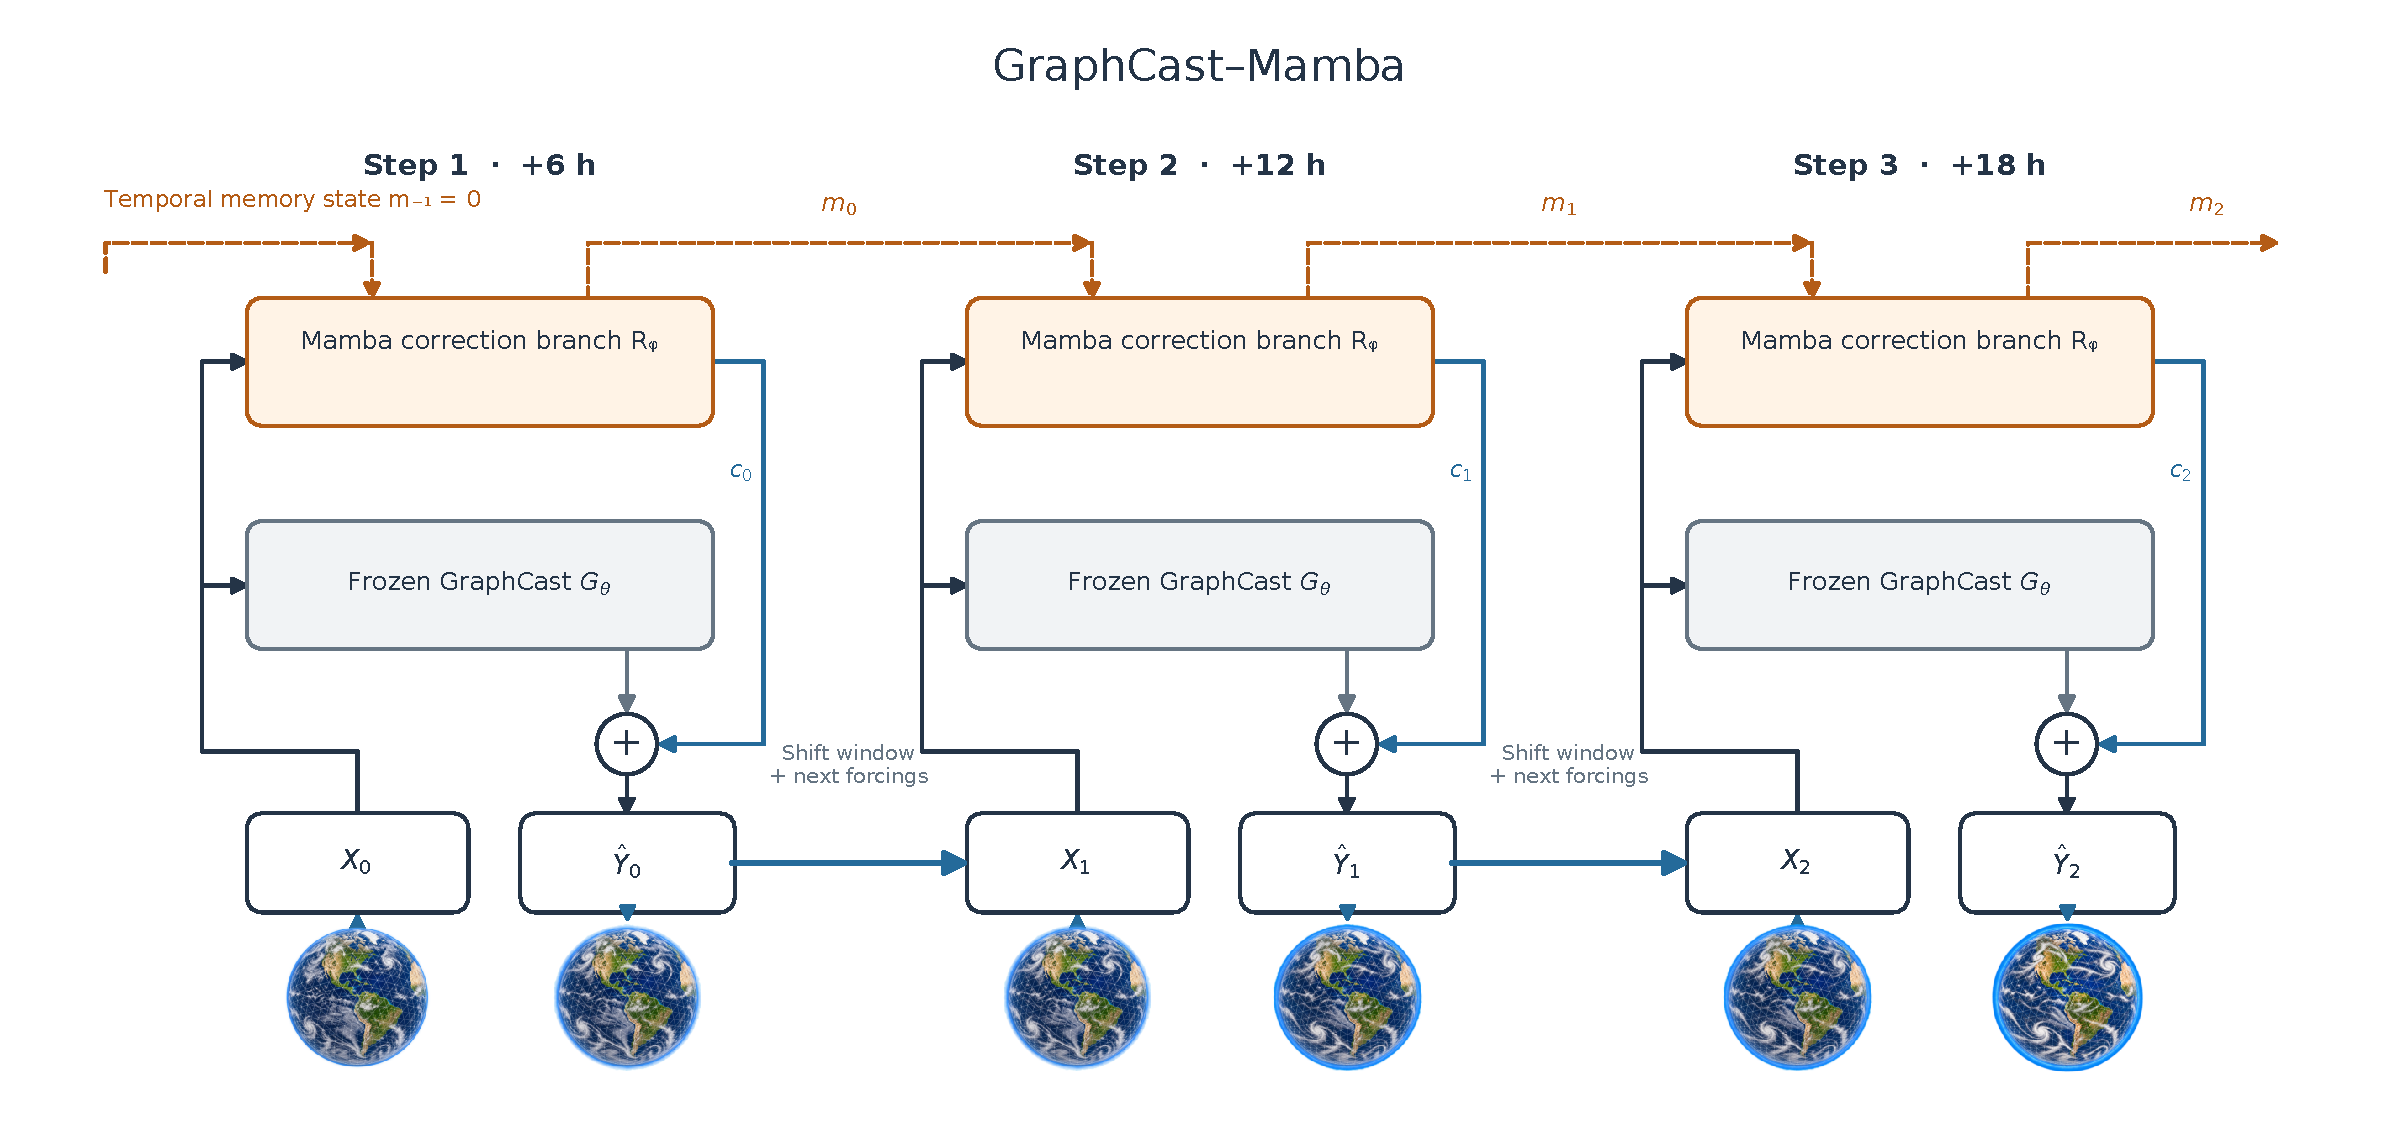
\includegraphics[width=\linewidth]{Pics/gc_mamba_architecture/03_temporal_rollout.pdf}
    \caption{Closed-loop autoregressive forecasting carries information along
    two paths. The combined weather prediction updates the next two-frame input
    window, with known forcings advanced to the next step. Separately, Mamba
    states and convolution caches pass between successive correction calls
    (dashed orange arrows). The illustrated cold-start rollout initializes
    temporal memory to zero and uses six-hour forecast steps. Model parameters
    are shared across forecast steps, and the GraphCast baseline remains frozen.}
    \label{fig:gc_mamba_temporal_rollout}
\end{figure}
